%-----------------------------------------------------------------------
%
%   UFRJ  - Universidade Federal do Rio de Janeiro
%   COPPE - Coordena��o dos Programas de P�s-gradua��o em Engenharia
%   PEE   - Programa de Engenharia El�trica
%
%   COE-835  Controle adaptativo
%
%   Relat�rio da simula��o
%                                                         Ramon R. Costa
%                                                         05/out/09, Rio
%-----------------------------------------------------------------------
\documentclass[11pt,a4paper]{article}
\usepackage[latin1]{inputenc} %pacote para utilizar palavras acentuadas
\usepackage{amsmath,amssymb}  %pacotes do AMS
\usepackage{latexsym}         %pacote para incluir s�mbolos (ex.\Box)
\usepackage{fancybox,fancyhdr}%pacote com frescuras
\usepackage{graphicx}         %pacote para incluir figuras tipo eps
\usepackage[portuguese]{babel}
\usepackage{xcolor}
\usepackage{float} 
\usepackage{epstopdf}
\usepackage[inline]{enumitem}
\usepackage[a4paper]{hyperref}% Make sure it comes last of your loaded packages
\hypersetup{
  verbose,
  plainpages=false,
  bookmarks=true,
  colorlinks=true,
  linkcolor=blue
}
     
%----------------------------------------------------------------------
%
%   Macros utilizados no LATEX
%                                                       Ramon R. Costa
%                                                       13/out/17, Rio
%----------------------------------------------------------------------
\newcount\m
\newcount\n

\def\twodigits#1{\ifnum #1<10 0\fi \number#1}

\def\hours{\n=\time \divide\n 60
    \m=-\n \multiply\m 60 \advance\m \time
    \twodigits\n:\twodigits\m}

\def\hora{\hours}

\def\fim{
  \medskip
  \begin{center}
    \rule[1mm]{30mm}{0.14mm}$\diamond$\rule[1mm]{30mm}{0.14mm}
  \end{center}
}

%----------------------------------------------------------------------
% A4 paper size & margins
\setlength {\textheight}    {25cm}%
\setlength {\textwidth}     {17.5cm}%
\setlength {\parindent}     {0mm}%
\setlength {\parskip}       {1mm}%
\setlength {\topmargin}     {-14mm}%
\setlength {\oddsidemargin} {-6mm}%
\setlength {\evensidemargin}{-6mm}%
\setlength {\columnsep}     {6mm}%

%----------------------------------------------------------------------
\def\codigo{COE-835}
\def\disciplina{Controle adaptativo}
\def\periodo{3o. período/2017}
\def\professor{Ramon}

\newcommand{\BOX}[1]{
  \framebox{{\color{magenta}\rule[-3mm]{1mm}{9mm}} ~~$\displaystyle
  \begin{aligned} #1 \end{aligned}$~~}\pagestyle{plain}
}

\newcommand{\RED}[1]{\colorbox{white}{\textcolor{red}{#1}}}
%\newcommand{\WoR}[1]{\colorbox{red}{\textcolor{white}{#1}}}
\newcommand{\BLU}[1]{\colorbox{white}{\textcolor{blue}{#1}}}
\newcommand{\GRE}[1]{\colorbox{green}{\textcolor{black}{#1}}}
\newcommand{\HI}[1]{\colorbox{yellow}{\textcolor{black}{#1}}}  %% Highlithed text

\newcommand{\estrela}[1]{
  \def\TXT{\RED{$\bigstar$ }}
  \hspace*{5mm}\TXT \hfill
  \parbox[t]{ \textwidth - \widthof{\TXT} - 5mm}{#1}
  \par
}

\def\Ltwo{\mbox{${\mathcal L}_2$}}
\def\Linf{\mbox{${\mathcal L}_\infty$}}

\newcommand{\sign}{\mbox{sign}}

\newcommand{\equacao}[2]{
  \makebox[40mm][l]{#1 \dotfill}: \quad \parbox[t]{8cm}
	{\begin{equation} \displaystyle
  \begin{aligned}
    #2
  \end{aligned} \end{equation}} \\
}

\newcommand{\sref}[1]{Section~\ref{#1}}
\newcommand{\fref}[1]{Fig.~\ref{#1}}
\newcommand{\tref}[1]{Table~\ref{#1}}
\newcommand{\thref}[1]{Theorem~\ref{#1}}
\newcommand{\aref}[1]{Assumption~\ref{#1}}
\newcommand{\norm}[1]{\left\lVert#1\right\rVert}
%\renewcommand{\qedsymbol}{}
\newcommand{\rev}[1]{{\color{red}#1}}
%\newcommand{\mat}[1]{\begin{bmatrix}#1\end{bmatrix}}

\newtheorem{remark}{Remark}
\newtheorem{lemma}{Lema}

%----------------------------------------------------------------------


%Set normal paragraph spacing
\setlength\parindent{24pt}

\begin{document}
%---------------------------------------------------------------------
\pagestyle{fancy}%
\renewcommand{\headrulewidth}  {0.4pt}%
\renewcommand{\footrulewidth}  {0.4pt}%
\lhead{\bfseries{Relat�rio do Trabalho 6}}%
\chead{}%
\rhead{\bfseries\thepage}%
\lfoot{}%
\cfoot{}%
\rfoot{[\hours] \quad \today}%
%---------------------------------------------------------------------
\begin{center}
  \huge{COE-835  Controle  adaptativo}  \\[20mm]

  \Large{Trabalho 6} \\[20mm]
\end{center}

\textbf{Grupo:} \quad \parbox[t]{10cm}{
Guilherme Pires Sales de Carvalho \\[2mm]
Matheus Ferreira dos Reis \\[2mm]
Renan Salles de Freitas \\[10mm]
}

\textbf{Algoritmo:} \quad \HI{MRAC Direto} ($n^* = 2$) \\[2mm]

\bigskip%
\textbf{Caso}: \quad \parbox[t]{10cm}{
  $n = 2, 3$ \quad (ordem da planta) \\[2mm]
  $n^* = 2$ \quad (grau relativo) \\[2mm]
  $n_p = 4, 6$ \quad (\# de par�metros) \\[15mm]
}

%---------------------------------------------------------------------
\tableofcontents
\newpage
%---------------------------------------------------------------------
%---------------------------------------------------------------------
\section{MRAC direto para plantas de grau relativo 2}

Uma das principais hip�teses utilizadas na demonstra��o de estabilidade do algoritmo MRAC direto para plantas de $n^* = 1$ � a 
necessidade do modelo de referencia escolhido ser uma fun��o de transfer�ncia SPR. Isto � necess�rio para que a lei de adapta��o 
seja formulada como fun��o apenas do erro de estima��o do sistema.
%
Para o algoritmo do MRAC direto para plantas de maior grau relativo, n�o � poss�vel escolher um modelo de refer�ncia $M(s)$ que 
seja SPR. Portanto, Monopoli \cite{} prop�s um m�todo para estender o algoritmo MRAC direto para $n^* = 2$, que consiste em escolher 
um polin�mio $L(s) = s+\alpha$ tal que $M(s)\,L(s)$ seja SPR.

A estrutura do controlador � id�ntica ao caso $n^* = 1$, cujo diagrama em blocos foi repetido aqui para maior clareza:
%
\begin{figure}[H]
  \centering
  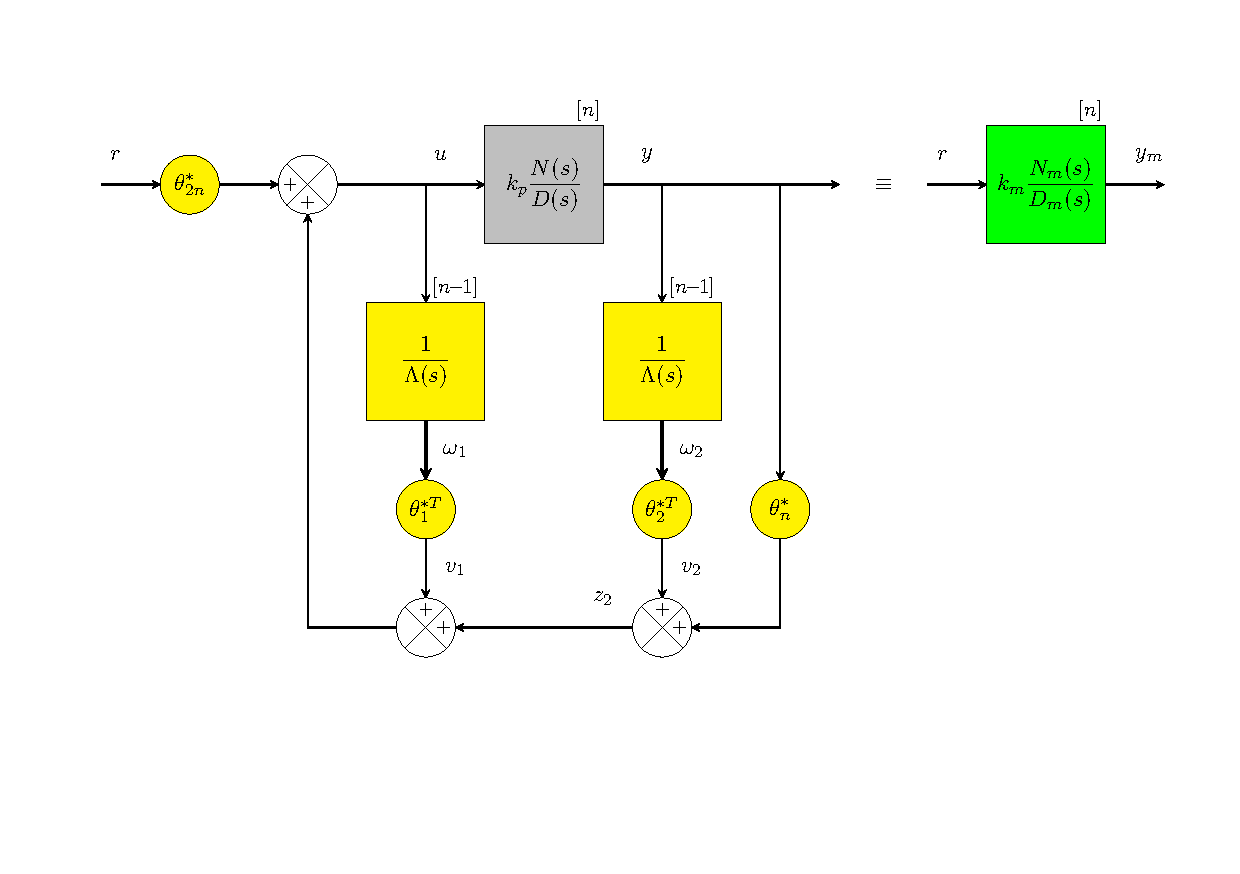
\includegraphics[width=15cm]{figs/mrac.pdf}
  \caption{Estrutura MRAC.}
  \label{mrac} 
\end{figure}

O algoritmo de adapta��o resultante, bem como a prova de estabilidade do mesmo s�o muito parecidos com o caso $n^* = 1$, e ser�o otimidos aqui por conveni�ncia. A id�ia b�sica consiste em utilizar os sinais $\chi = L^{-1}\,u$ como um novo controle e o regressor filtrado $\zeta = L^{-1}\,\omega$ como um novo regressor para o sistema.
%
Assim, � poss�vel mostrar que a lei de adapta��o 
%
\begin{equation}
\dot{\theta}(t) = -\textrm{sign}[k_p] \, \Gamma \, \zeta(t) \, e(t),
\label{eq:adaptation}
\end{equation}
%
em conjunto com a lei de controle 
%
\begin{equation}
u(t) = \theta^\intercal\omega + \dot{\theta}^\intercal\omega
\label{eq:control}
\end{equation}
%
garantem a estabilidade assint�tica dos erros de estima��o e sa�da do sistema realimentado. Note que o sinal $\dot{\theta}$ presente em \eqref{eq:control} pode ser implementado na pr�tica devido � sua defini��o na lei de adapta��o \eqref{eq:adaptation}. Substituindo \eqref{eq:adaptation} em \eqref{eq:control}, a forma completa da lei de controle � dada por:

\begin{equation}
u(t) = \theta^\intercal\omega - \textrm{sign}[k_p] \, \Gamma \, e(t) \, \zeta^{\intercal}\omega
\label{eq:control2}
\end{equation}

Neste trabalho, ser�o consideradas plantas de segunda e terceira ordens com grau
relativo 2 ($n^*=2$). Iremos simular e discutir o comportamento do erro e das
sa�das para varia��es das condi��es iniciais dos par�metros estimados
($\theta(0)$) e da planta ($y(0)$), do ganho de adapta��o $\Gamma$ e para
diferentes par�metros da planta e modelo.

%Considere um sistema linear invariante no tempo descrito pela equa��o
%diferencial (Eq. \ref{eq:planta}):
%%
%\begin{equation}
%P(s) \, [y](t) = Z(s) \, [u](t),
%\label{eq:planta}
%\end{equation}
%
%onde $y(t) \in \mathbb{R}$ e $u(t) \in \mathbb{R}$ s�o os sinais medidos de
%sa�da e entrada do sistema, sendo:
%%
%\begin{gather}
%P(s) = s^n + p_{n-1}s^{n-1}+\ldots + p_1s+p_0\,\\
%Z(s) = z_ms^m + z_{m-1}s^{m-1}+\ldots + z_1s+z_0 \,,
%\label{eq:poly}
%\end{gather}
%%
%os polin�mios em $s$, com $s$ sendo o operador de diferencial
%$s[x](t)=\dot{x}(t)$. $p_i$, $i = 0,1,\ldots,n-1$ e $z_i$, $i=0,1,\ldots,m$ ($n>m$) s�o os par�metros desconhecidos da planta.
%
%O objetivo do controle �: dado um modelo de refer�ncia, descrito como
%
%\begin{equation}
%P_m(s)[y_m](t) = r(t),
%\end{equation}
%
%onde $P_m(s)$ � um polin�mio est�vel m�nico e $r(t)$ � a entrada de refer�ncia
%limitada, encontrar uma lei de controle $u(t)$ tal que todo o sistema de malha
%fechada produza sinais limitados e a sa�da da planta $y(t)$ rastreie o modelo
%de refer�ncia $y_m(t)$ assintoticamente. A estrutura exige algumas premissas:
%\begin{enumerate}
  %\item $Z(s)$ � um polin�mio est�vel (planta � de fase m�nima);
  %\item O sinal de $k_p$ � conhecido;
  %\item O grau relativo da planta � conhecido;
  %\item A ordem da planta � conhecida.
	%\item O modelo de referencia � dado por uma fun��o de transfer�ncia SPR.
%\end{enumerate}
%
%A estrutura do controlador � 2DOF, como pode ser visto na figura
%\ref{mrac}. Escolhe-se ent�o um polin�mio est�vel $\Lambda(s) =
%s^n+\lambda_{n-1}s^{n-1}+\ldots+\lambda_1s+\lambda_0$ para filtrar a entrada e a
%sa�da da planta com o filtro $\frac{1}{\Lambda(s)}$. A equa��o do controlador
%� descrita como:
%\begin{equation}
%u(t) = \theta_1^\intercal\omega_1(t)+\theta_2^\intercal\omega_2(t)+\theta_n
%y(t)+ \theta_{2n} r(t),
%\end{equation}
%
%onde o filtro � descrito pela realiza��o de estados:
%
%\begin{gather}
%\dot{\omega}_1(t) = A_\lambda \, \omega_1(t) + bu(t)\,,\\
%\dot{\omega}_2(t) = A_\lambda \, \omega_2(t) + by(t)\,,
%\label{eq:statespace}
%\end{gather}
%%
%onde $\omega_1(t) \in \mathbb{R}^n$, $\omega_2(t) \in \mathbb{R}^n$ e:
%%
%\begin{equation}
%A_\lambda = 
%\begin{bmatrix}
    %0      & 1      & 0      & \dots  & 0      & 0      \\
    %0      & 0      & 1      & 0      & \dots  & 0      \\
    %\vdots & \vdots & \vdots & \vdots & \vdots & \vdots \\
    %0      & 0      & \dots  & \dots  & 0      & 1      \\
    %-\lambda_0 & -\lambda_1 & \dots & \dots & -\lambda_{n-2} & -\lambda_{n-1} 
%\end{bmatrix}
%\in \mathbb{R}^{n \times n} \,, \quad b =
%\begin{bmatrix}
    %0  \\
    %\vdots  \\
    %0 \\
    %1 \\ 
%\end{bmatrix}
%\in \mathbb{R}^n \,.
%\label{eq:statespace}
%\end{equation}
%
%\begin{figure}[H]
  %\centering
  %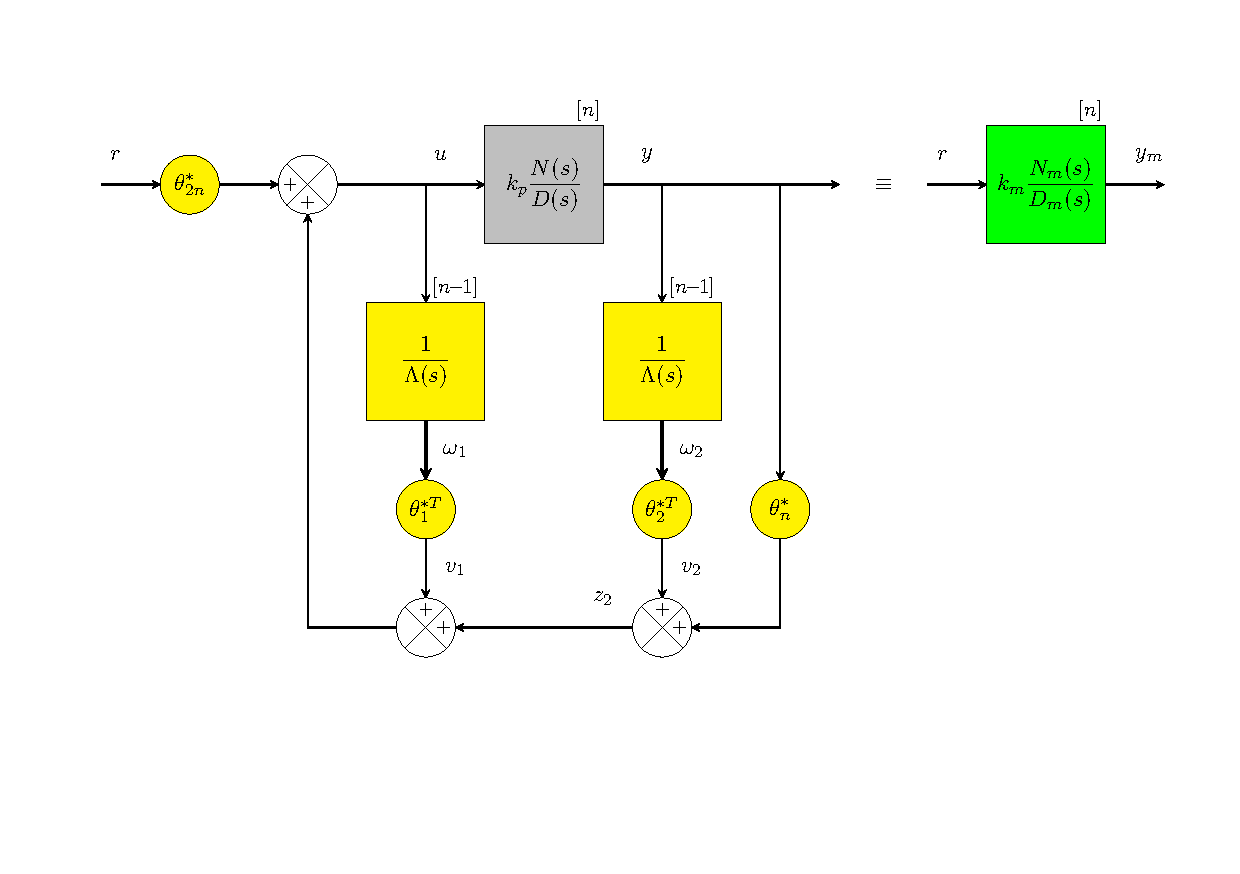
\includegraphics[width=15cm]{figs/mrac.pdf}
  %\caption{Estrutura MRAC.}
  %\label{mrac} 
%\end{figure}
%
%Os valores ideais para o controle $\theta^*$ podem ser obtidos como j�
%descrito no trabalho 4, se os par�metros da planta fossem conhecidos. Como n�o �
%o caso, consideramos $\theta$ como uma estimativa dos par�metros ideais e
%formulamos a lei de controle:
%
%\begin{gather}
%u(t) = \theta^\intercal\omega, \\
%\omega(t) = \left[\omega_1(t)^\intercal \quad y(t) \quad \omega_2(t)^\intercal
%\quad r(t)\right]^\intercal, \\
%\theta = \left[\theta_1 \quad \theta_n \quad \theta_2 \quad \theta_{2n}\right]
%\end{gather}
%
%Definindo o erro como $e(t) = y(t) - y_m(t)$, � poss�vel demonstrar por
%Lyapunov que, variando $\theta$ atrav�s da lei de adapta��o
%
%\begin{equation}
%\dot{\theta}(t) = -\textrm{sign}[k_p] \, \Gamma \, \omega(t) \, e(t),
%\end{equation}
%%
%o erro converge assintoticamente para zero, quando $\Gamma =
%\Gamma^\intercal > 0$ � uma matriz de ganhos positiva definida.

%\section{Implementa��o}


%---------------------------------------------------------------------
\section{Resultados das simula��es}

%Simula��o utilizando \HI{\texttt{Matlab/Simulink}}.

%\subsection{Gradiente Normalizado}

Nas simula��es, procuramos avaliar o comportamento do sistema para as seguintes condi��es:
%
\begin{enumerate*}[label=(\roman*)]
\item condi��es iniciais $\theta(0)$ e $y(0)$;
\item Par�metros da planta e do modelo;
\item ganho de adapta��o $\Gamma$.
\end{enumerate*}

Apresentaremos os resultados obtidos atrav�s de simula��es no ambiente \HI{\texttt{Matlab/Simulink}} e os discutiremos na pr�xima se��o.

\subsection{Simula��o \#1}

Inicialmente, verificamos o comportamento do sistema para varia��es no \textbf{par�metro de adapta��o} $\Gamma$.

\bigskip

\textbf{\underline{Simula��o 1.1}: sistema de 2$^\text{a}$ ordem}
%
\begin{align*}
  y &= \frac{1}{s^2-2s+1}u \,, &  y_m &=
  \frac{1}{s^2+3s+2}r\,, & A_0 &= s+1,\\ \theta(0) &= \mathbf{0} \,, & y(0) &= \textbf{0} \,, & L(s) &= s+1.5 \\ L(s) &= s+1.5 \\
  \gamma &= \HI{200} \textbf{I}_4 \,, \, \textrm{e} \, \HI{20} \, \textbf{I}_4\,,
  & r &= 10\textrm{sin}(2t) + 25\textrm{sin}(3t) \, .
\end{align*}

\begin{figure}[H]
  \centering
  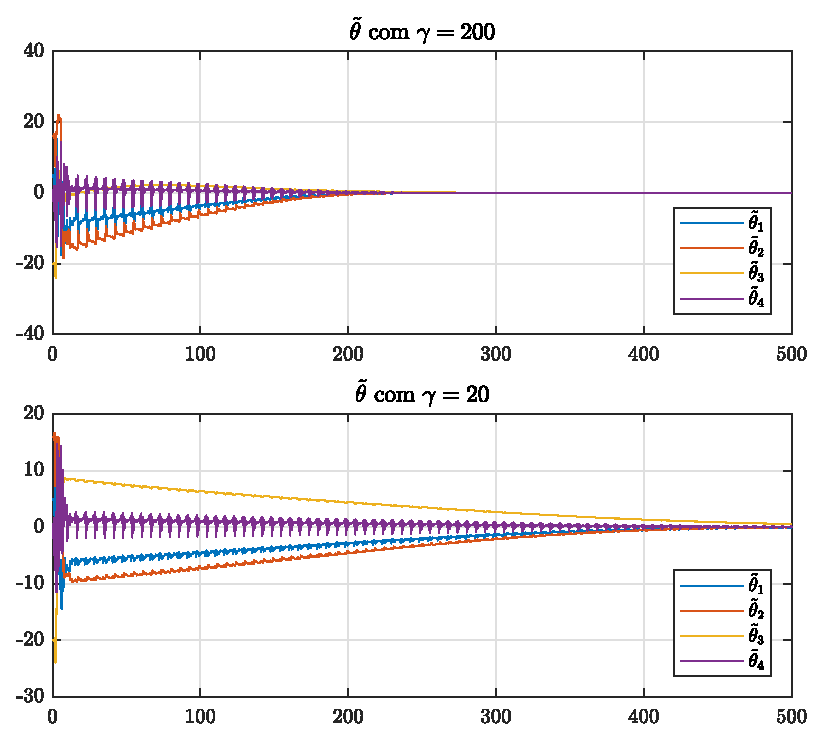
\includegraphics[width=12cm]{figs/tiltheta/sim02_gamma200gamma20.eps}
\end{figure}

\begin{figure}[H]
  \centering
  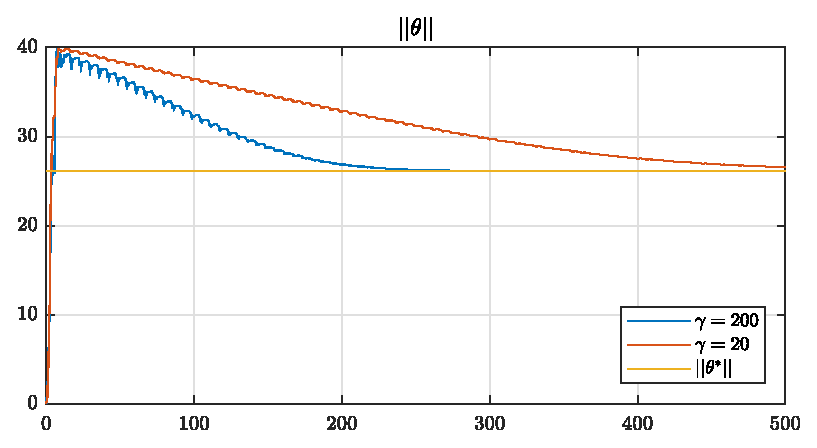
\includegraphics[width=12cm]{figs/modtheta/sim02_gamma200gamma20.eps}
\end{figure}

\begin{figure}[H]
  \centering
  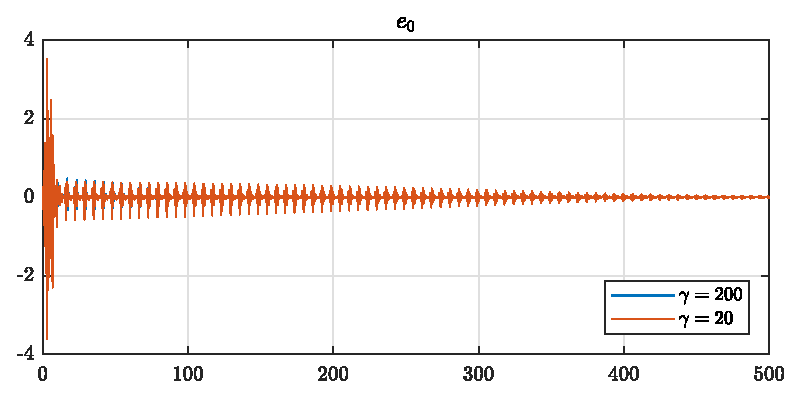
\includegraphics[width=12cm]{figs/e0/sim02_gamma200gamma20.eps}
\end{figure}

\bigskip

\textbf{\underline{Simula��o 1.2}: sistema de 3$^\text{a}$ ordem}
%
\begin{align*}
  y &= \frac{s+1}{s^3-6s^2+12s-8}u \,, &  y_m &=
  \frac{s+0.8}{s^3+3s^2+2.75s+0.75}r\,, & A_0 &= s+1,\\ \theta(0) &= \mathbf{0} \,, & y(0) &= \textbf{0} \,, & L(s) &= s+1.5 \\
  \gamma &= \HI{200} \textbf{I}_6 \,, \, \textrm{e} \, \HI{20} \, \textbf{I}_6\,, & r &= 10\textrm{sin}(2t) + 25\textrm{sin}(3t) + 10\textrm{sin}(5t) \, .
\end{align*}

\begin{figure}[H]
  \centering
  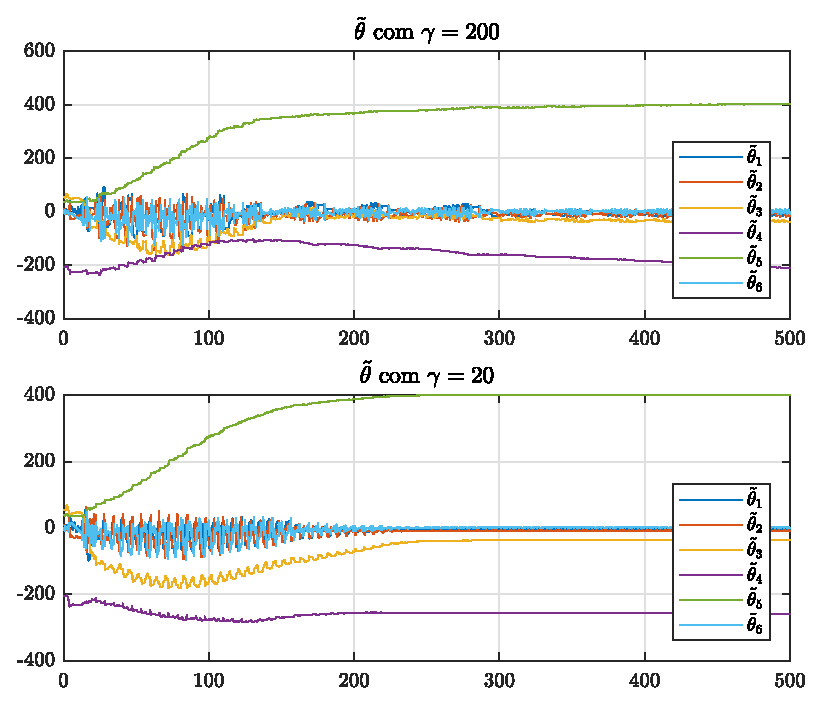
\includegraphics[width=12cm]{figs/tiltheta/sim03_gamma200gamma20.eps}
\end{figure}

\begin{figure}[H]
  \centering
  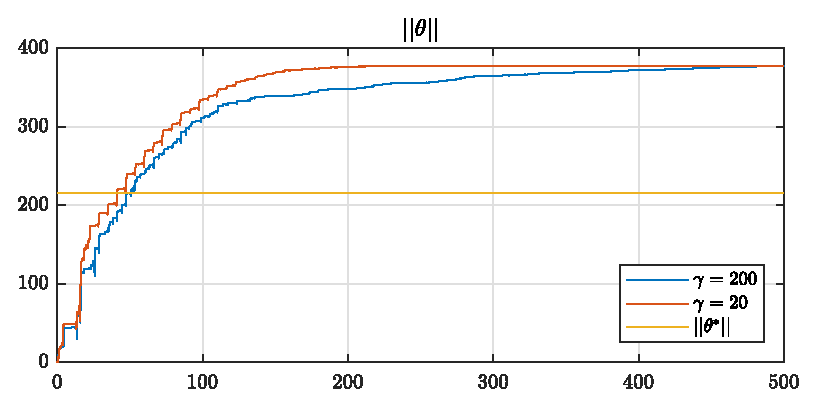
\includegraphics[width=12cm]{figs/modtheta/sim03_gamma200gamma20.eps}
\end{figure}

\begin{figure}[H]
  \centering
  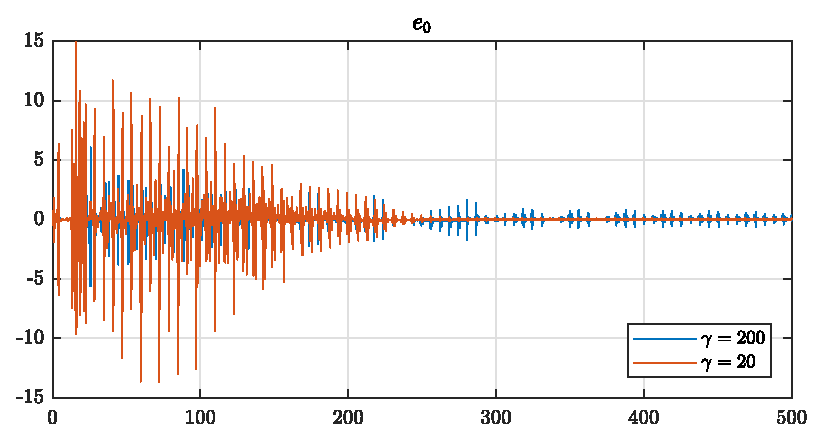
\includegraphics[width=12cm]{figs/e0/sim03_gamma200gamma20.eps}
\end{figure}

%---------------------------------------------------------------------

\subsection{Simula��o \#2}

Verificamos agora o comportamento do sistema para varia��es na \textbf{condi��o inicial} $y(0)$.

\bigskip

\textbf{\underline{Simula��o 2.1}: sistema de 2$^\text{a}$ ordem}
%
\begin{align*}
  y &= \frac{1}{s^2-2s+1}u\,,  &  y_m &= \frac{1}{s^2+3s+2}r\,, & A_0 &= s+1,\\ \theta(0) &= \mathbf{0} \,, & y(0) &= \HI{$\mathbf{0}$ \,, $\mathbf{10}$} \,,  & L(s) &= s+1.5 \\
  \gamma &= 200 \, \textbf{I}_4\,, & r &= 10\textrm{sin}(2t) + 25\textrm{sin}(3t) \, .
\end{align*}

\begin{figure}[H]
  \centering
  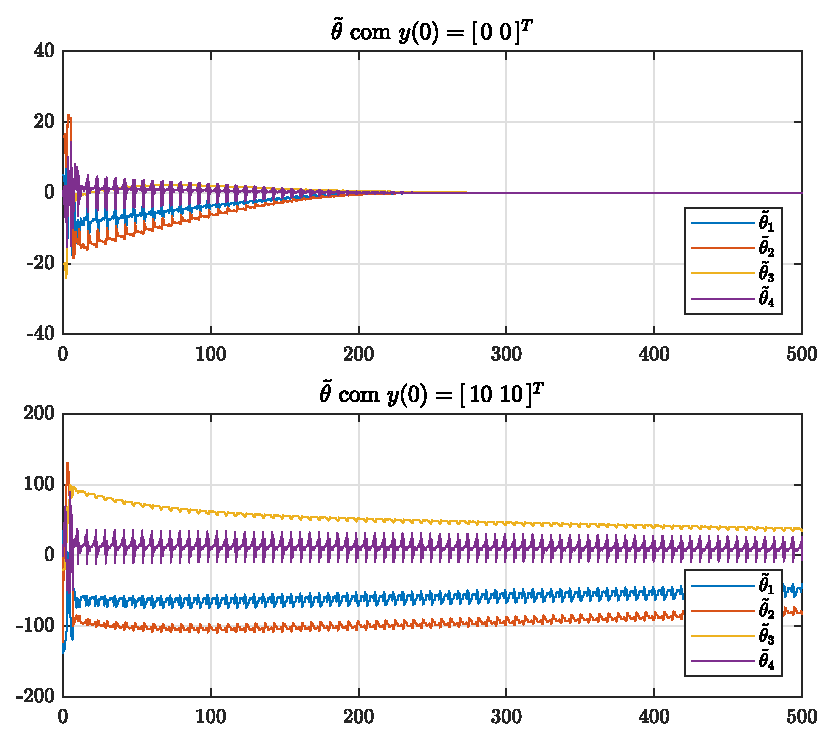
\includegraphics[width=12cm]{figs/tiltheta/sim02_y01y02.eps}
\end{figure}

\begin{figure}[H]
  \centering
  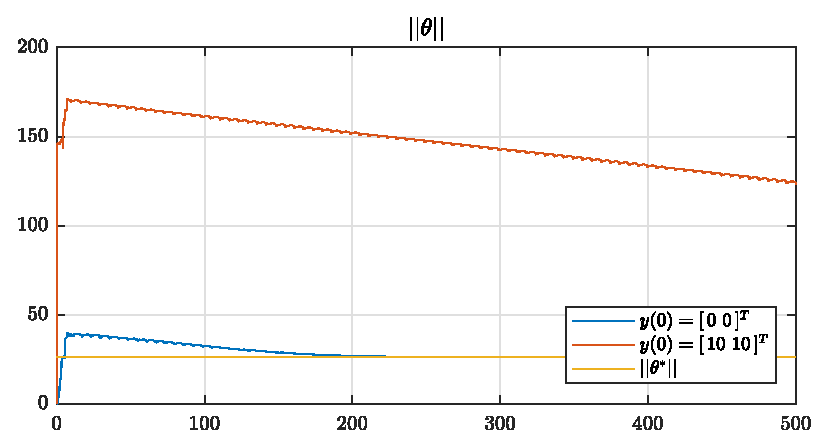
\includegraphics[width=12cm]{figs/modtheta/sim02_y01y02.eps}
\end{figure}

\begin{figure}[H]
  \centering
  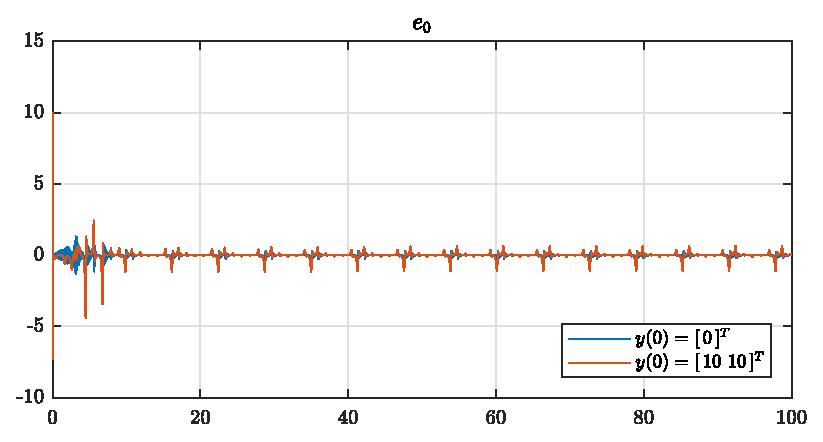
\includegraphics[width=12cm]{figs/e0/sim02_y01y02.eps}
\end{figure}

\bigskip

\textbf{\underline{Simula��o 2.2}: sistema de 3$^\text{a}$ ordem}
%
\begin{align*}
  y &= \frac{s+1}{s^3-6s^2+12s-8}u \,, &  y_m &=
  \frac{s+0.8}{s^3+3s^2+2.75s+0.75}r\,, & A_0 &= s+1,\\ \theta(0) &= \mathbf{0} \,, & y(0) &= \HI{$\mathbf{0}$ \,, $\mathbf{10}$} \,,  & L(s) &= s+1.5 \\
  \gamma &= 200 \textbf{I}_6 \,, & r &= 10\textrm{sin}(2t) + 25\textrm{sin}(3t) + 10\textrm{sin}(5t) \, .
\end{align*}

\begin{figure}[H]
  \centering
  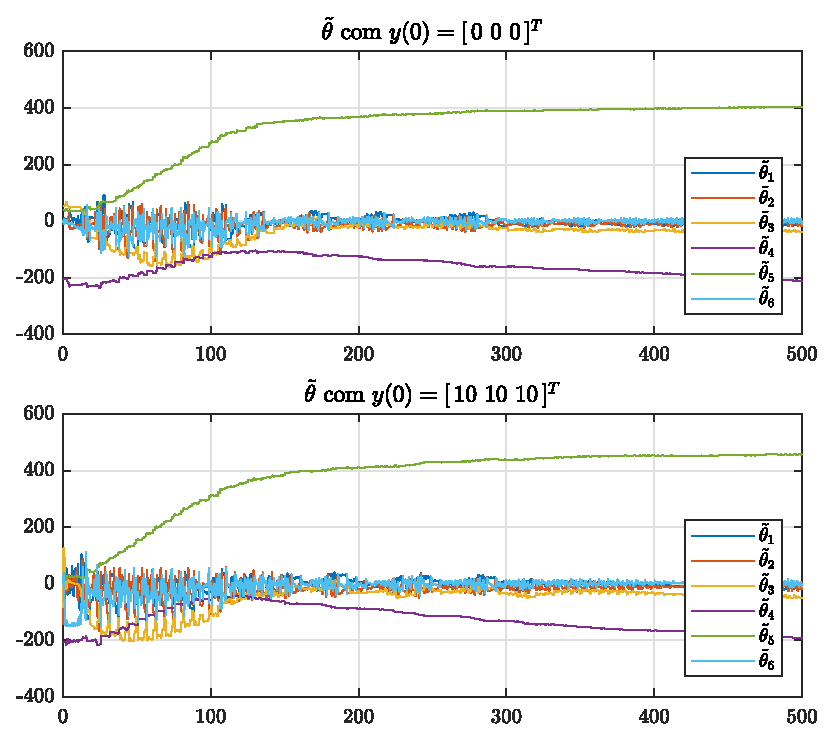
\includegraphics[width=12cm]{figs/tiltheta/sim03_y01y02.eps}
\end{figure}

\begin{figure}[H]
  \centering
  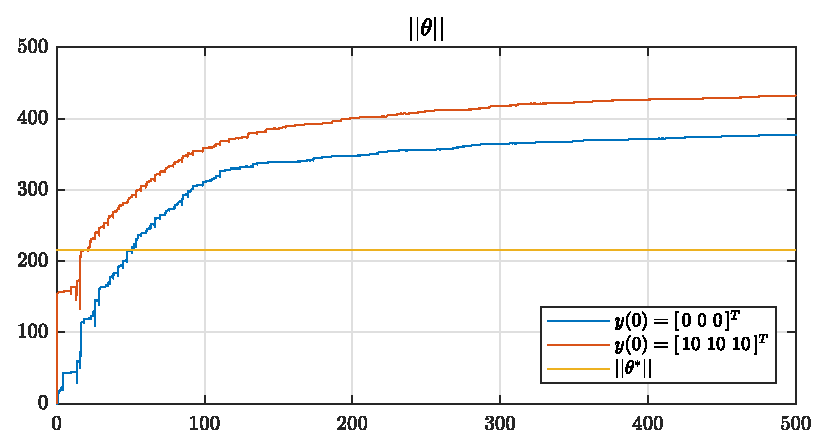
\includegraphics[width=12cm]{figs/modtheta/sim03_y01y02.eps}
\end{figure}

\begin{figure}[H]
  \centering
  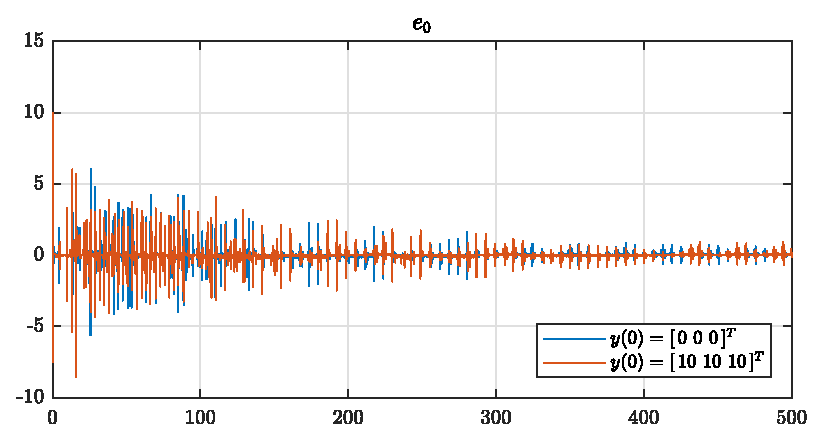
\includegraphics[width=12cm]{figs/e0/sim03_y01y02.eps}
\end{figure}

% -----------------------------------------------------------------------------

\subsection{Simula��o \#3}

Verificamos o comportamento do sistema para varia��es na \textbf{fun��o de transfer�ncia da planta} $P(s)$.

\bigskip

\textbf{\underline{Simula��o 3.1}: sistema de 2$^\text{a}$ ordem}
%
\begin{align*}
  y &= \HI{$\frac{1}{s^2-2s+1}u$}\,, \HI{$\frac{2}{s^2+7s+12}u$}\,,  &  y_m &=
  \frac{1}{s^2+3s+2}r\,, & A_0 &= s+1,\\ \theta(0) &= \textbf{0} \,, & y(0) &= \textbf{0} \,, & L(s) &= s+1.5 \\
  \gamma &= 200 \, \textbf{I}_4\,, & r &= 10\textrm{sin}(2t) + 25\textrm{sin}(3t) \, .
\end{align*}

\begin{figure}[H]
  \centering
  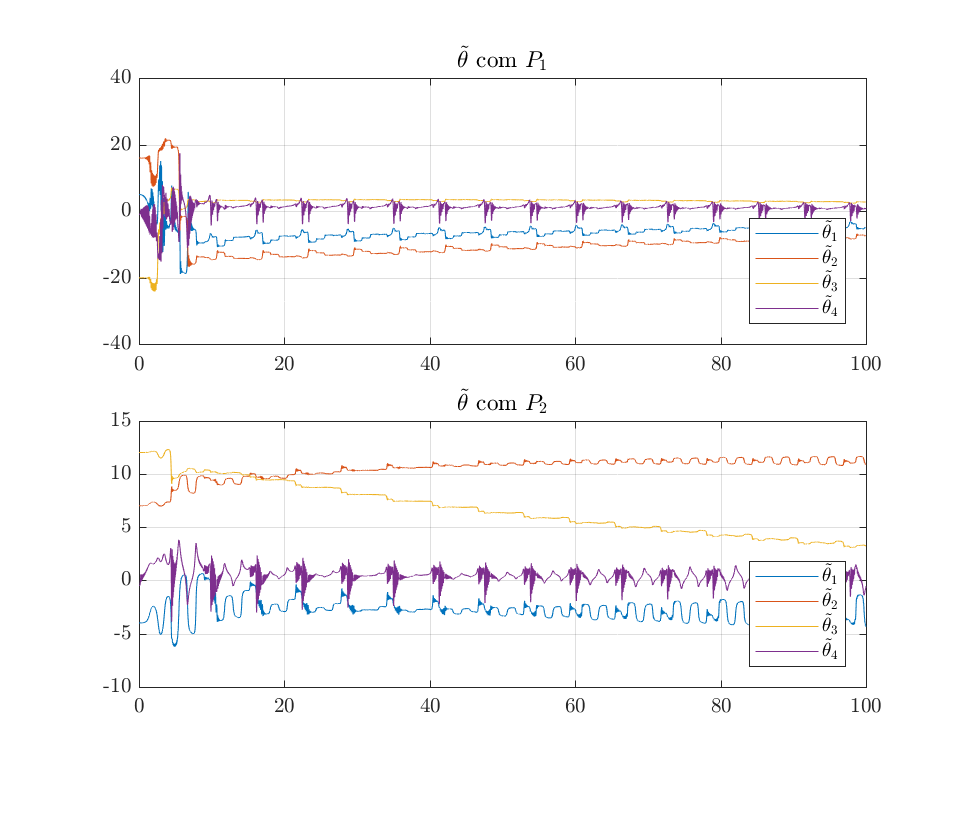
\includegraphics[width=12cm]{figs/tiltheta/sim02_P1P2.eps}
\end{figure}

\begin{figure}[H]
  \centering
  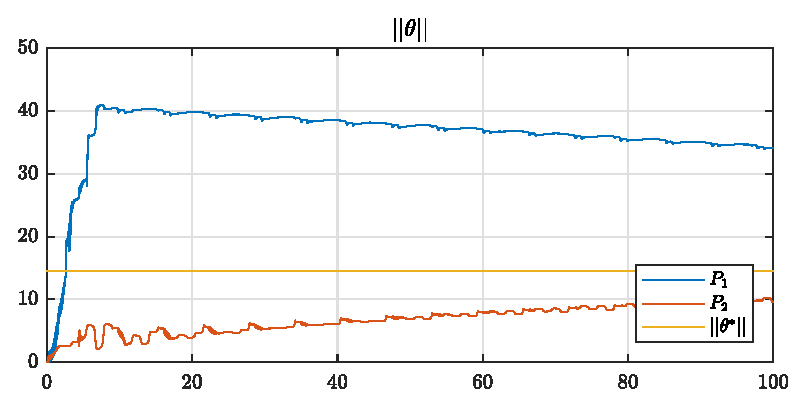
\includegraphics[width=12cm]{figs/modtheta/sim02_P1P2.eps}
\end{figure}

\begin{figure}[H]
  \centering
  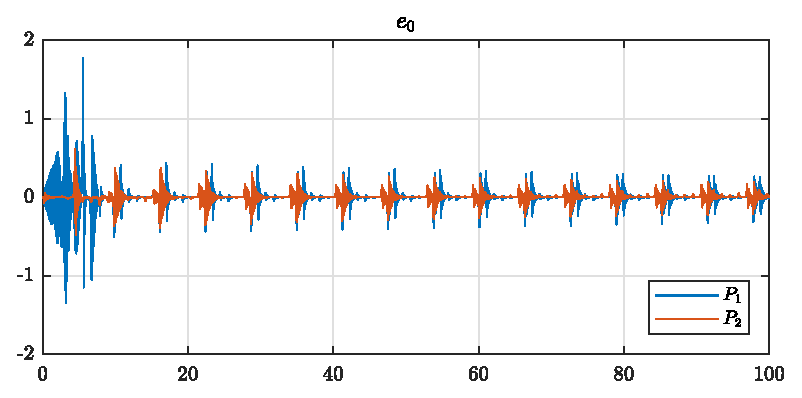
\includegraphics[width=12cm]{figs/e0/sim02_P1P2.eps}
\end{figure}

\textbf{\underline{Simula��o 3.2}: sistema de 3$^\text{a}$ ordem}
%
\begin{align*}
  y &= \HI{$\frac{s+1}{s^3-6s^2+12s-8}u$}\,, \HI{$\frac{2s+4}{s^3+6s^2+11s+6}u$}\,,  &  y_m &=
  \frac{s+0.8}{s^3+3s^2+2.75s+0.75}r\,, & A_0 &= s+1,\\ \theta(0) &= \textbf{0} \,, & y(0) &= \textbf{0} \,, & L(s) &= s+1.5 \\
  \gamma &= 200 \, \textbf{I}_6\,, & r &= 10\textrm{sin}(2t) + 25\textrm{sin}(3t) + 10\textrm{sin}(5t) \, .
\end{align*}

\begin{figure}[H]
  \centering
  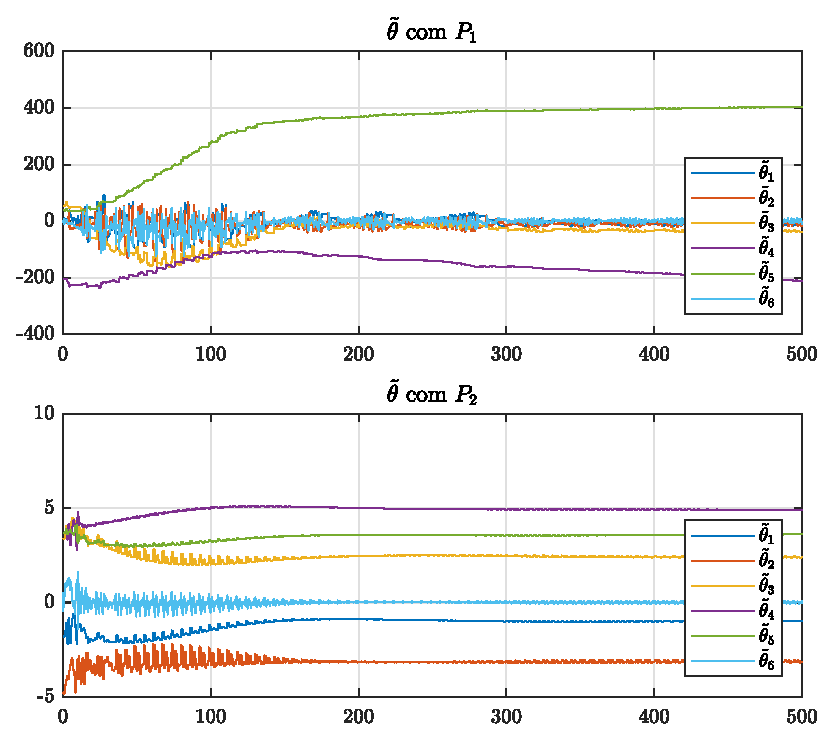
\includegraphics[width=12cm]{figs/tiltheta/sim03_P1P2.eps}
\end{figure}

\begin{figure}[H]
  \centering
  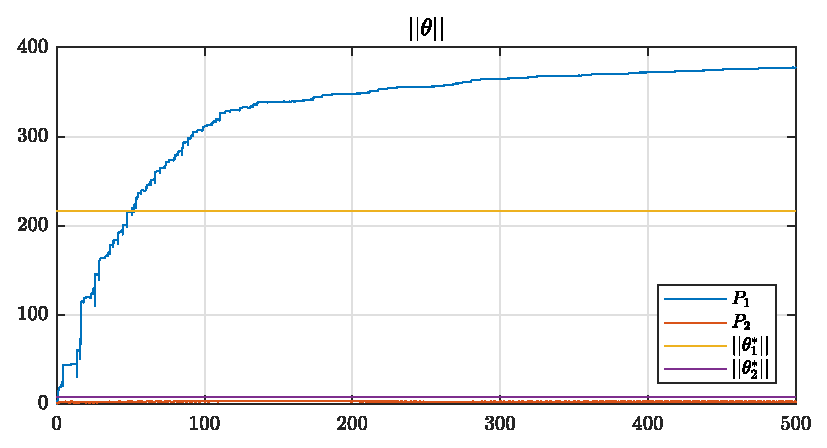
\includegraphics[width=12cm]{figs/modtheta/sim03_P1P2.eps}
\end{figure}

\begin{figure}[H]
  \centering
  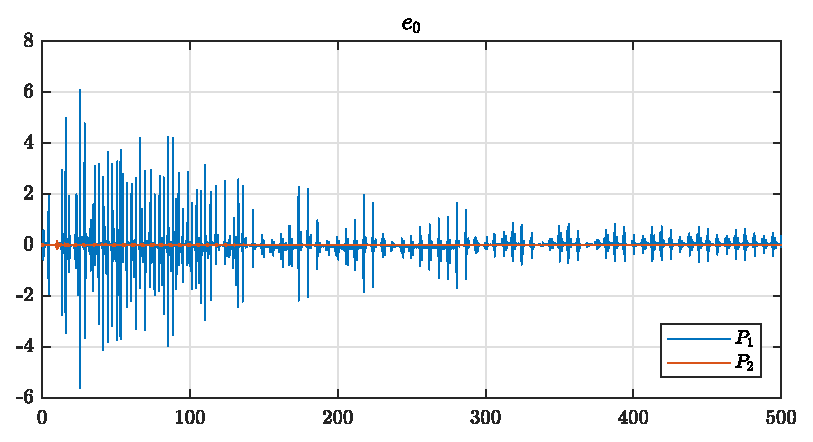
\includegraphics[width=12cm]{figs/e0/sim03_P1P2.eps}
\end{figure}

% -----------------------------------------------------------------------------

\subsection{Simula��o \#4}

Verificamos o comportamento do sistema para varia��es na \textbf{fun��o de transfer�ncia do modelo de refer�ncia} $P_m(s)$.

\bigskip

\textbf{\underline{Simula��o 4.1}: sistema de 2$^\text{a}$ ordem}
%
\begin{align*}
  y &= \frac{1}{s^2-2s+1}u \,,  &  y_m &= \HI{$\frac{1}{s^2+3s+2}r$}\,, \HI{$\frac{1}{s^2+5s+6}r$ }\,, & A_0 &= s+1,\\ \theta(0) &= \textbf{0} \,, & y(0) &= \textbf{0} \,, & L(s) &= s+1.5 \\
  \gamma &= 200 \, \textbf{I}_4\,, & r &= 10\textrm{sin}(2t) + 25\textrm{sin}(3t) \, .
\end{align*}

\begin{figure}[H]
  \centering
  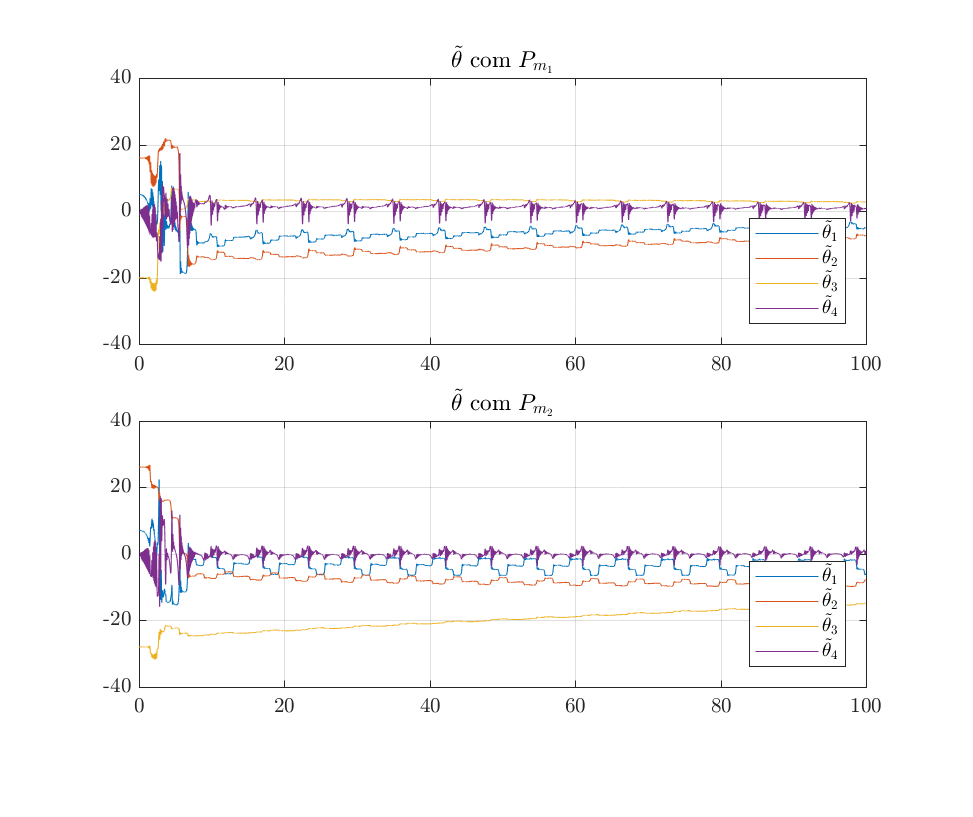
\includegraphics[width=12cm]{figs/tiltheta/sim02_Pm1Pm2.eps}
\end{figure}

\begin{figure}[H]
  \centering
  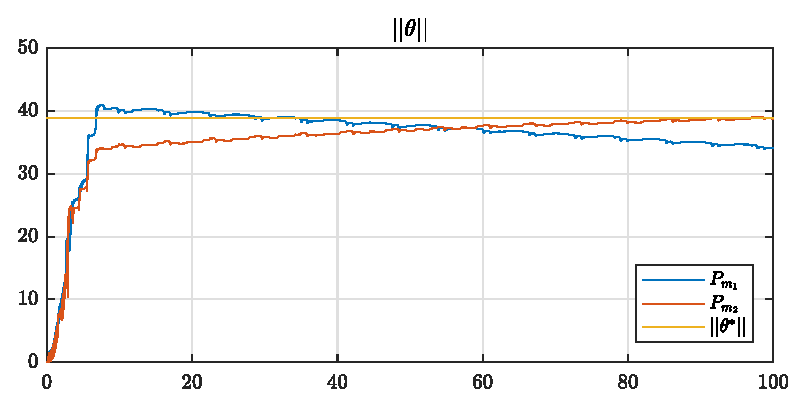
\includegraphics[width=12cm]{figs/modtheta/sim02_Pm1Pm2.eps}
\end{figure}

\begin{figure}[H]
  \centering
  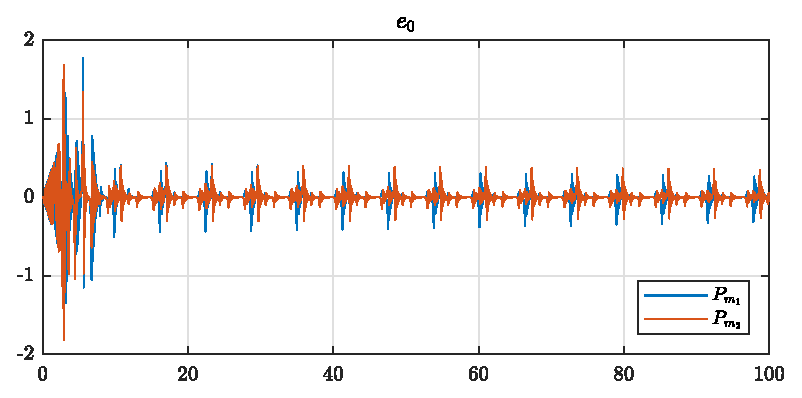
\includegraphics[width=12cm]{figs/e0/sim02_Pm1Pm2.eps}
\end{figure}

\textbf{\underline{Simula��o 4.2}: sistema de 3$^\text{a}$ ordem}
%
\begin{align*}
  y &= \frac{s+1}{s^3-6s^2+12s-8}u \,,  &  y_m &= \HI{$\frac{s+0.8}{s^3+3s^2+2.75s+0.75}r$}\,, \HI{$\frac{s+1.5}{s^3+5.5s^2+8.5s+3}r$ }\,, & A_0 &= s+1,\\ \theta(0) &= \textbf{0} \,, & y(0) &= \textbf{0} \,, & L(s) &= s+1.5 \\
  \gamma &= 200 \, \textbf{I}_6\,, & r &= 10\textrm{sin}(2t) + 25\textrm{sin}(3t) + 10\textrm{sin}(5t) \, .
\end{align*}

\begin{figure}[H]
  \centering
  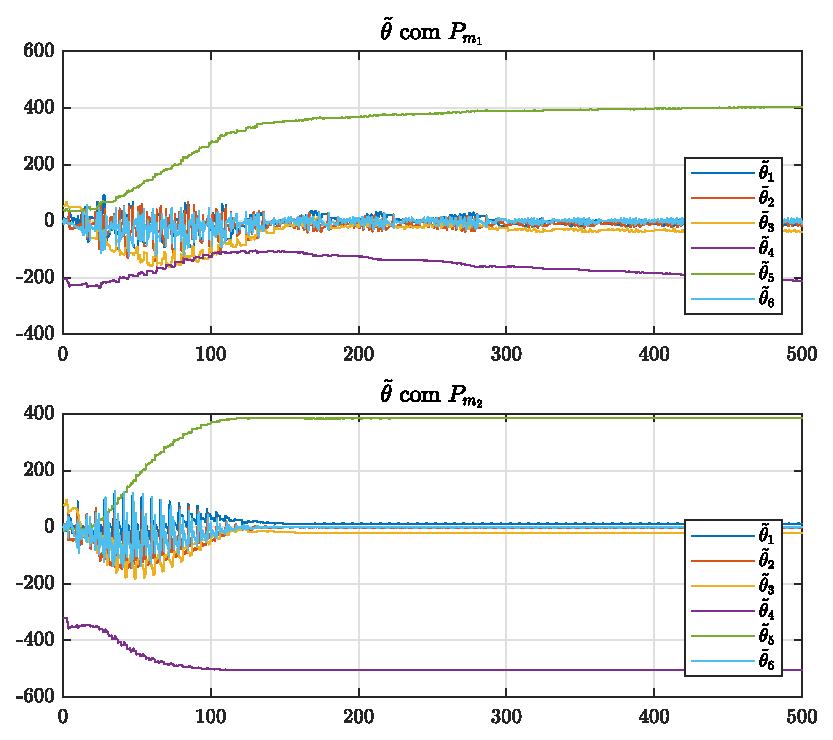
\includegraphics[width=12cm]{figs/tiltheta/sim03_Pm1Pm2.eps}
\end{figure}

\begin{figure}[H]
  \centering
  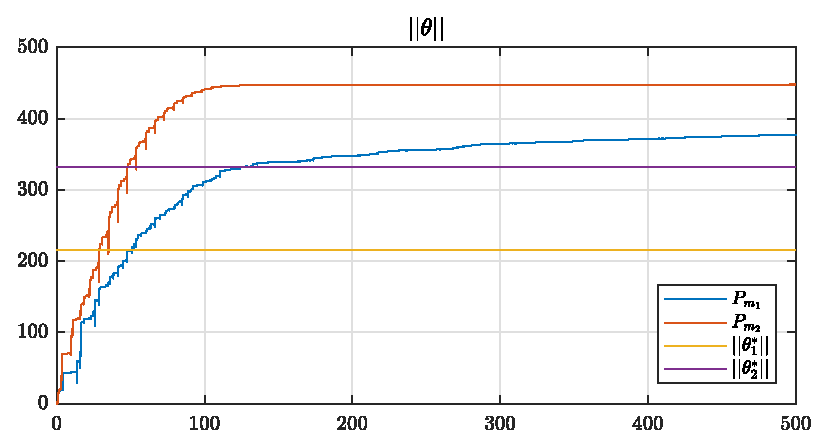
\includegraphics[width=12cm]{figs/modtheta/sim03_Pm1Pm2.eps}
\end{figure}

\begin{figure}[H]
  \centering
  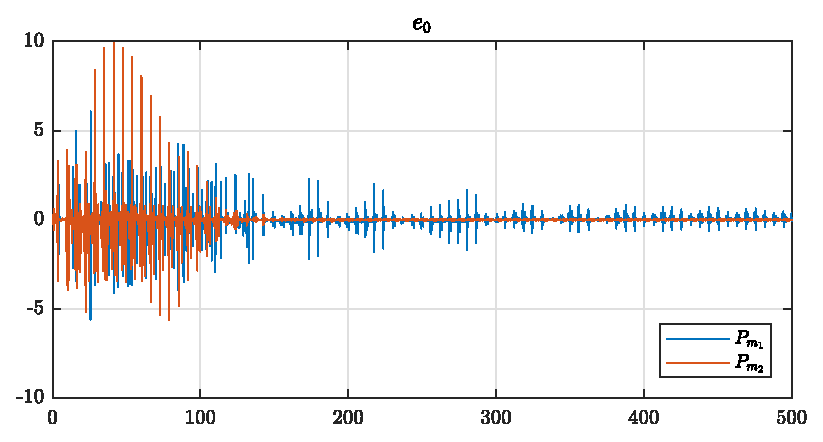
\includegraphics[width=12cm]{figs/e0/sim03_Pm1Pm2.eps}
\end{figure}
% \newpage
%---------------------------------------------------------------------
\section{Discuss�o}

Os resultados apresentados neste trabalho s�o semelhantes aos apresentados nos trabalhos anteriores sobre MRAC, s� que aplicado a sistemas de primeira ordem. Neste trabalho, s�o abordados sistemas de segunda e terceira ordens com grau relativo 2. O polin�mio $A_0(s)$ foi definido como $s+1$ e o multiplicador de Monopoli como $L(s) = s+1.5$ para todas as simula��es. Os sinais de refer�ncia foram escolhidos de modo a ter o n�mero de frequ�ncias necess�rias para haver excita��o persistente.

A \textbf{simula��o \#1} mostra o comportamento do sistema para varia��es no
ganho de adapta��o $\Gamma$. Para o sistema de $2^a$ ordem escolhido, um ganho maior resultou em uma estima��o mais r�pida dos par�metros, convergindo para os reais. Para o sistema de $3^a$ ordem, o desempenho foi semelhante entre os dois ganhos, e em ambos os casos o vetor de par�metros entrou em quadratura com o regressor. No entanto, os erros de sa�da convergiram para zero em todos os casos.

A \textbf{simula��o \#2} mostra o comportamento do sistema para varia��es na condi��o inicial $y(0)$. Como previsto, condi��es iniciais da planta mais longe em rela��o �s condi��es iniciais do modelo de refer�ncia resultam em um transit�rio muito maior, o que � um problema conhecido de controle adaptativo.

A \textbf{simula��o \#3} apresenta o comportamento do sistema para varia��es na fun��o de transfer�ncia da planta $P(s)$. Nota-se que o controle encontra maior dificuldade em fazer uma planta com din�mica mais r�pida rastrear um modelo de refer�ncia mais lento.

Finalmente, na \textbf{simula��o \#4}, os modelos de refer�ncia $P_m(s)$ foram variados e verificou-se que, escolhendo um modelo de refer�ncia com din�mica mais r�pida, a converg�ncia � mais lenta para a planta de segunda ordem. J� para a planta de terceira ordem, a converg�ncia foi mais r�pida para o modelo de refer�ncia com din�mica mais r�pida.
%---------------------------------------------------------------------
%\bibliographystyle{agsm}
%\bibliography{bib,coe736}

%---------------------------------------------------------------------
\end{document}
